% compile this on sharelatex.com
% !TEX program = pdflatex

\documentclass[a4paper]{scrartcl}
\usepackage[utf8]{inputenc}
\usepackage{graphicx}
\usepackage{float}
\usepackage{dsfont}
\usepackage{amsmath,amsthm}
\usepackage{lmodern}
\usepackage{subfigure}
\usepackage{enumerate}
\usepackage{geometry}

\geometry{a4paper,left=30mm,right=30mm, top=2cm, bottom=2.5cm}

\title{Submission Sheet 3}
\author{Danny Heinrich \and Matthias Kasperidus \and Leonard Kleinhans}
\date{26. November 2014}

\newcommand*\colvec[2]{
        \begin{pmatrix} #1 \\ #2 \end{pmatrix}
}

\begin{document}
\maketitle

\section{Exercise 3.1: Fuzzy Sets}

One can determine whether something is a book or a poem by counting the words of a piece. A crisp set for the amount of words used would be $X=[1,130000]$ since the average amount of words used in a book is about 130.000. For the age we define a crisp set over $Y = [0,100]$ , since anyone older than 100 would certainly be an old person as well as a grown up, which would be the same for the age of 70 in our point of view. The last set should be measured by its number of people. We define the last crisp set $Z=[1,60]$. We then proceeded to define the membership functions as we saw fit for our examples.

\begin{align*}
 N(x)&=\begin{cases}
    0, & \text{if $x<500 \vee x>5000$}.\\
    -\frac{((x-500) \cdot (x-5000))}{5062500}, &        \text{otherwise}.
    \end{cases} \\
 B(x)&=\begin{cases}
    0, & \text{if $x<500 \vee x>5000$}.\\
    1, & \text{if $x>10000$}. \\
    \frac{x}{6500}-\frac{7}{13}, & \text{otherwise}.
  \end{cases} \\
    P(x)&=\begin{cases}
        0, & \text{if $x<0 \vee x>1000$}.\\
        -\frac{((x-0) \cdot (x-1000))}{250000}, & \text{otherwise}.
    \end{cases}
\end{align*}

\begin{align*}
 Y(x)&=\begin{cases}
     \frac{x}{14} - \frac{4}{7}, & \text{if $x>=8 \wedge x<22$}.\\
    -\frac{x}{8}+\frac{15}{4}, & \text{if $x>=22 \wedge x<30$}. \\
    0, & \text{otherwise}.
    \end{cases} \\
 C(x)&=\begin{cases}
    \frac{x}{8}, & \text{if $x>=0 \wedge x<8$}.\\
    -\frac{x}{6}+\frac{7}{3}, & \text{if $x>=8 \wedge x<=14$}. \\
    0, & \text{otherwise}.
  \end{cases} \\
  O(x)&=\begin{cases}
    0, & \text{if $x<40$}.\\
    1, & \text{if $x>70$}. \\
    \frac{x}{30}-\frac{4}{3}, & \text{otherwise}.
    \end{cases}\\
 G(x)&=\begin{cases}
    0, & \text{if $x<18$}.\\
    1, & \text{if $x>30$}. \\
    \frac{x}{12}-\frac{3}{2}, & \text{otherwise}.
    \end{cases}
\end{align*}

\begin{align*}
 Gr(x)&=\begin{cases}
    \frac{x}{5}-1, & \text{if $x>=5 \wedge x<10$}.\\
    -\frac{x}{10}+2, & \text{if $x>=10 \wedge x<20$}. \\
    0, & \text{otherwise}.
    \end{cases} \\
 Cl(x)&=\begin{cases}
    \frac{x}{10}-2, & \text{if $x>=20 \wedge x<30$}.\\
    -\frac{x}{20}+\frac{5}{2}, & \text{if $x>=30 \wedge x<=50$}. \\
    0, & \text{otherwise}.
  \end{cases} \\
    Cr(x)&=\begin{cases}
        0, & \text{if $x<30$}.\\
        1, & \text{if $x>100$}. \\
        \frac{x}{70}-\frac{3}{7}, & \text{otherwise}.
    \end{cases}
\end{align*}


We illustrated the functions above as follows. Beginning at the top the functions are named after the shorthand of their respective Sets e.g. N stands for Newspaper Article and G stands for Grown Up and so on.

\begin{figure}[H]
    \centering
    \subfigure[Words]{
        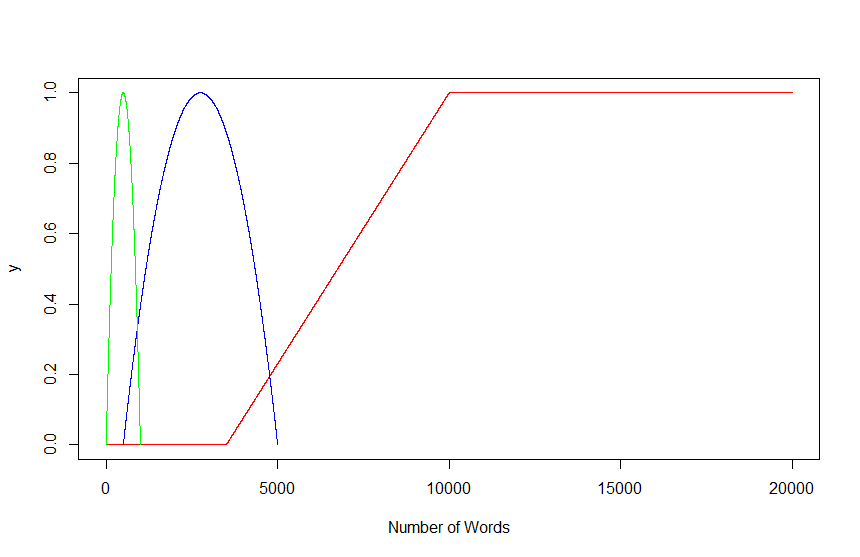
\includegraphics[width=0.44\textwidth]{img/FuzzyWords}
    }  
    \quad
    \subfigure[Age]{
        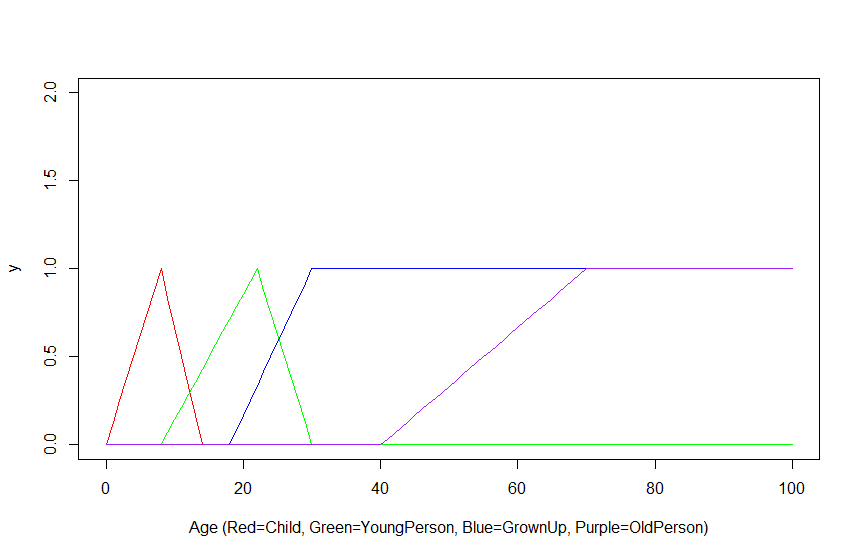
\includegraphics[width=0.44\textwidth]{img/FuzzyAge}
    }
    \quad
    \subfigure[Number of People]{
        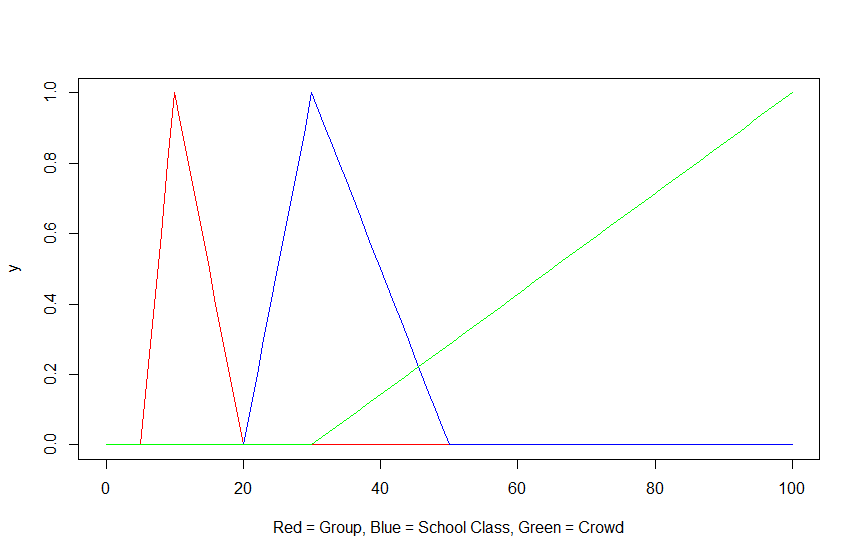
\includegraphics[width=0.44\textwidth]{img/FuzzyPeople}
    }   

\caption{Fuzzy Sets over given Examples}
\end{figure}	

\begin{figure}[H]
    \centering
    \subfigure[Book and Newspaper Article]{
        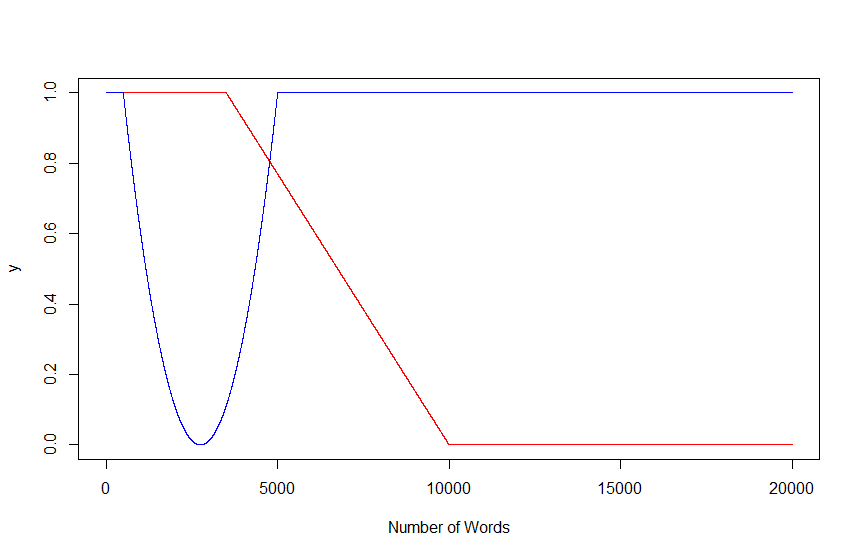
\includegraphics[width=0.44\textwidth]{img/ComplementWords}
    }  
    \quad
    \subfigure[Child and Young Person]{
        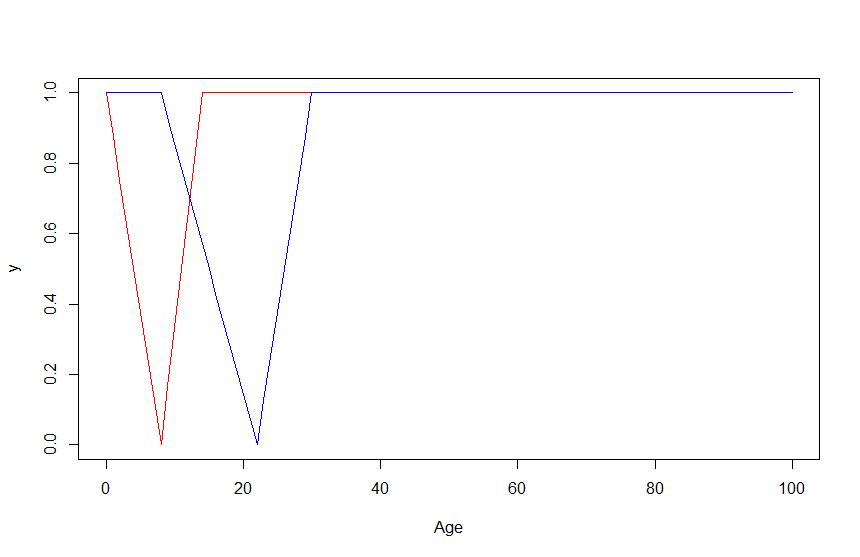
\includegraphics[width=0.44\textwidth]{img/ComplementAge}
    }
\caption{Complement of two sets.}
\end{figure}	

\begin{figure}[H]
    \centering
    \subfigure[Book and Article]{
        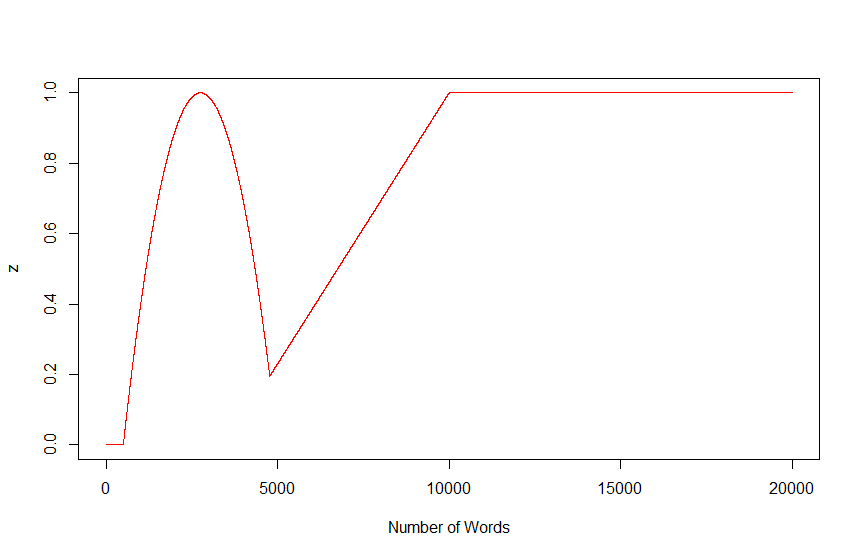
\includegraphics[width=0.44\textwidth]{img/UnionWords}
    }  
    \quad
    \subfigure[Child and Young Person]{
        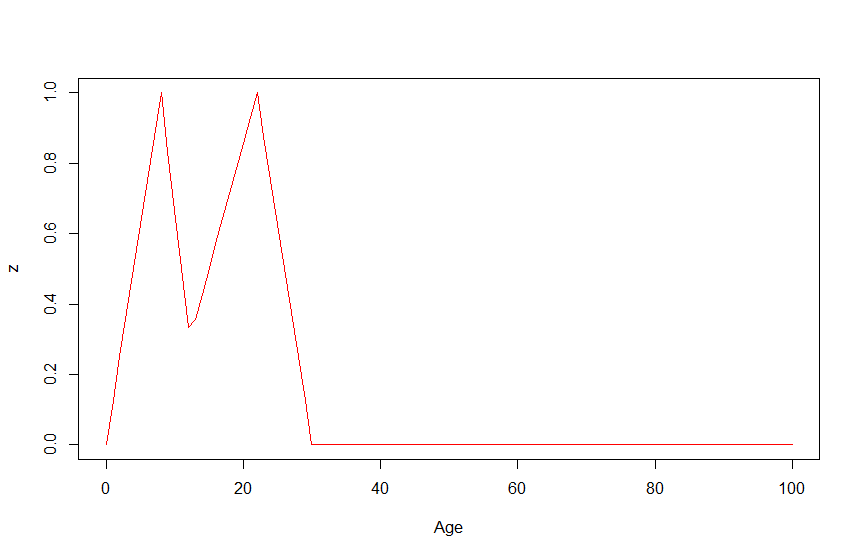
\includegraphics[width=0.44\textwidth]{img/UnionAge}
    }
\caption{Union of two sets.}
\end{figure}	

\begin{figure}[H]
    \centering
    \subfigure[Book and Article]{
        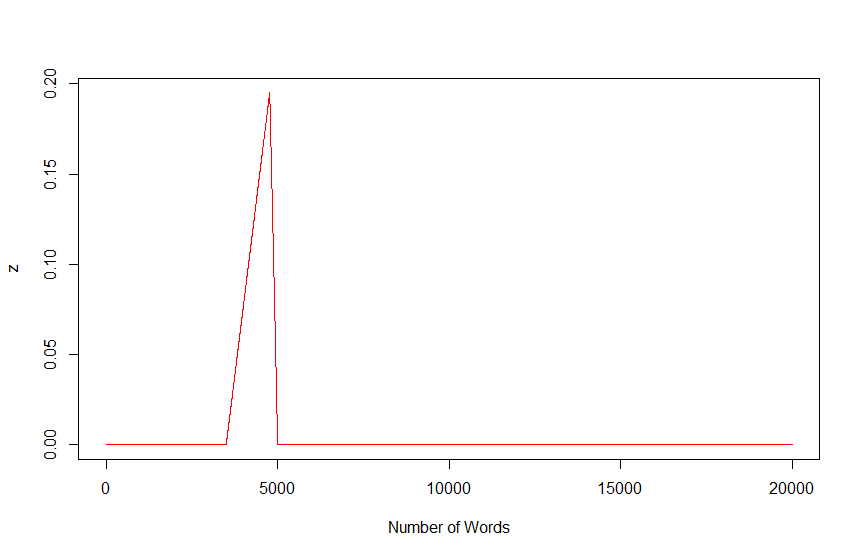
\includegraphics[width=0.44\textwidth]{img/IntersectionWords}
    }  
    \quad
    \subfigure[Child and Young Person]{
        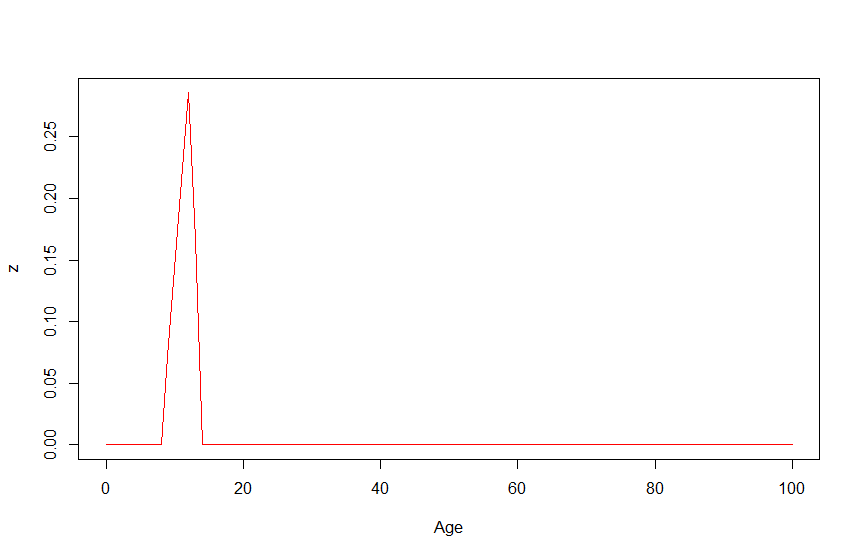
\includegraphics[width=0.44\textwidth]{img/IntersectionAge}
    }
\caption{Intersection of two sets.}
\end{figure}


\section{Exercise 3.2: Fuzzy Complements}
As defined in lecture a fuzzy complement obtained from an arbitrary increasing generator is a function $c: [0,1] \to [0,1]$ where
$\forall a \in [0,1]: c(a) = g^{(-1)}\left(g(1)-g(a)\right)$ and $\exists$ a continuous function $g:[0,1] \to \mathds{R}$ with $g(0) = 0$ and $g$ strictly monotone increasing. \\
\\

\textbf{To be proven:} $\forall a \in [0,1]: c(c(a)) = a$ \\
Because $g(0) = 0$, $g$ continuous and $g$ strictly monotone increasing, $g$ is bijective in [0,1] and the inverse function exists (in [0,1]).
\begin{align*}
        c(c(a)) &= c \left( g^{(-1)} \left( g(1) - g(a) \right) \right) \\
                &= g^{(-1)} \left( g(1) - g \left( g^{(-1)} \left( g(1) - g(a) \right) \right) \right) \\
                &= g^{(-1)} \left( g(1)-g(1)+g(a) \right) \\
                &= g^{(-1)} \left( g(a) \right) \\
                &= a 
\end{align*}
    
\qed

\section{Exercise 3.3: Dual Triples}
\textbf{To be proven:}
\begin{align*}
c\left( t(a, b) \right) &= s\left( c(a), c(b) \right) \\
c\left( s(a, b) \right) &= t\left( c(a), c(b) \right)
\end{align*}
\begin{enumerate}[a)]
\item 
    \begin{align*}
    c(t(a,b)) &= c(ab) = 1-ab \\
    s(c(a),c(b)) &= s(1-a,1-b) = 1-a +1 -b - (1-a) (1-b)\\
    &= 2 - a -b - 1 +a +b -ab  = 1-ab \\
    \\
    c(s(a,b)) &= c(a+b-ab) = 1 -a -b + ab \\
    t(c(a),c(b)) &= t(1-a,1-b) = 1-a-b+ab
    \end{align*}
    \qed
\item 
\begin{align*}
c(t(a,b)) &= c(\max\{0,a+b-1\}) = 1-\max\{0,a+b-1\} \\
s(c(a),c(b)) &= s(1-a,1-b) = \min \{1,2-a-b\} = - \max \{-1, a+b-2\} \\
&=  1-\max\{0,a+b-1\}\\
\\
 c(s(a,b)) &= c(\min \{1,a+b\} = 1 - \min \{ 1, a+b\} \\
 t(c(a),c(b)) &= t(1-a,1-b) = \max \{ 0, 1 - a -b\} = - \min \{ 0, a+b-1 \} \\ 
 &= 1 - \min\{1,a+b\}
\end{align*}
\qed

\end{enumerate}


\end{document}
